%; whizzy chapter
% -initex iniptex -latex platex -format platex -bibtex jbibtex -fmt fmt
% 以上 whizzytex を使用する場合の設定。

%     Kansai Debian Meeting resources
%     Copyright (C) 2007 Takaya Yamashita
%     Thank you for Tokyo Debian Meeting resources

%     This program is free software; you can redistribute it and/or modify
%     it under the terms of the GNU General Public License as published by
%     the Free Software Foundation; either version 2 of the License, or
%     (at your option) any later version.

%     This program is distributed in the hope that it will be useful,
%     but WITHOUT ANY WARRANTY; without even the implied warranty of
%     MERCHANTABILITY or FITNESS FOR A PARTICULAR PURPOSE.  See the
%     GNU General Public License for more details.

%     You should have received a copy of the GNU General Public License
%     along with this program; if not, write to the Free Software
%     Foundation, Inc., 51 Franklin St, Fifth Floor, Boston, MA  02110-1301 USA

%  preview (shell-command (concat "evince " (replace-regexp-in-string "tex$" "pdf"(buffer-file-name)) "&"))
% 画像ファイルを処理するためにはebbを利用してboundingboxを作成。
%(shell-command "cd image200708; ebb *.png")

%%ここからヘッダ開始。

\documentclass[mingoth,a4paper]{jsarticle}
\usepackage{kansaimonthlyreport}
\usepackage[dvips]{xy}


% 日付を定義する、毎月変わります。
\newcommand{\debmtgyear}{2009}
\newcommand{\debmtgmonth}{6}
\newcommand{\debmtgdate}{28}
\newcommand{\debmtgnumber}{24}

\begin{document}

\begin{titlepage}

% 毎月変更する部分、本文の末尾も修正することをわすれずに

 第\debmtgnumber{}回 関西 Debian 勉強会資料

\vspace{2cm}

\begin{center}
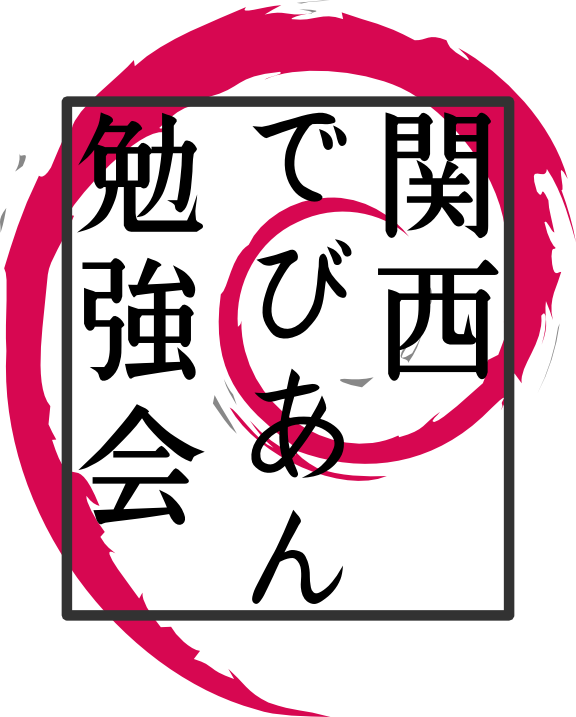
\includegraphics{image200802/kansaidebianlogo.png}
\end{center}

\begin{flushright}
\hfill{}関西 Debian 勉強会担当者 山下 尊也\\
\hfill{}\debmtgyear{}年\debmtgmonth{}月\debmtgdate{}日
\end{flushright}

\thispagestyle{empty}
\end{titlepage}

\dancersection{Introduction}{山下 尊也}
 
 関西 Debian 勉強会はDebian GNU/Linux のさまざ
 まなトピック(新しいパッケージ、Debian 特有の機能の仕組、Debian 界隈で起
 こった出来事、などなど)について話し合う会です。

 目的として次の三つを考えています。
 \begin{itemize}
  \item MLや掲示板ではなく、直接顔を合わせる事での情報交換の促進
  \item 定期的に集まれる場所
  \item 資料の作成
 \end{itemize}

 それでは、楽しい一時をお楽しみ下さい。

\newpage

\begin{minipage}[b]{0.2\hsize}
 {\rotatebox{90}{\fontsize{80}{80}
{\gt 関西デビアン勉強会}}}
\end{minipage}
\begin{minipage}[b]{0.8\hsize}
\hrule
\vspace{2mm}
\hrule
\setcounter{tocdepth}{1}
\tableofcontents
\vspace{2mm}
\hrule
\end{minipage}

\dancersection{ハッカーに一歩近づく Tips:Bash 編}{山下康成@京都府向日市}

\begin{table}[h]
\begin{center}
 \scriptsize
\caption{Bash コマンド一覧}
\begin{tabular}{|r|l|l|}
\hline
\multicolumn{3}{|c|}{<<コマンドの再実行>>}\\ \hline
1 & 以前実行したコマンドラインの呼出し &  上矢印キー、下矢印キー \\ \hline
2 & 以前実行したコマンドラインの呼出し & CTRL-P, CTRL-N \\ \hline
3 & 直前のコマンドの再実行 & !! \\ \hline
4 & 以前実行したコマンドラインに前方一致 & !(前方一致文字列) \\ \hline
5 & 以前実行したコマンドラインに部分一致 & !?(部分一致文字列) \\ \hline
6 & これまでに実行したコマンドラインの列挙 & history \\ \hline
7 & ヒストリ番号を用いた過去コマンド指定 & !(数字) \\ \hline
8 & 指定した回数前に実行したコマンド & !(負の数字) \\ \hline
9 & 実行されるコマンドの確認 & :p \\ \hline
\multicolumn{3}{|c|}{<<補完>>}\\ \hline
10 & パス名の補完 & TAB \\ \hline
11 & コマンドの補完 & TAB \\ \hline
\multicolumn{3}{|c|}{<<行編集>>}\\ \hline
12 & カーソルの左右移動 & CTRL-B/左矢印、CTRL-F/右矢印 \\ \hline
13 & カーソルの左の文字の消去 & BackSpace/Delete \\ \hline
14 & カーソルの行頭・行末への移動 & CTRL-A, CTRL-E \\ \hline
15 & カーソル位置の文字を消す & CTRL-D \\ \hline
16 & 行末まで消去 & CTRL-K \\ \hline
17 & 語頭まで消去 & CTRL-W \\ \hline
18 & 文字の入れ換え & CTRL-T \\ \hline
\multicolumn{3}{|c|}{<<直前のコマンドの一部を再利用する>>}\\ \hline
19 & 直前のコマンドの最後の引数 & !\$ \\ \hline
20 & 直前のコマンドの引数 & !* \\ \hline
21 & 直前のコマンドラインの一部を変更 & \^{ }A\^{ }B \\ \hline
22 & 直前のコマンドラインの一部を変更 & (以前のコマンド指定):s/A/B/ \\ \hline
\multicolumn{3}{|c|}{<<ワイルドカード>>}\\ \hline
23 & \.(ドット)で始まる以外に一致 & * \\ \hline
24 & 1文字に一致 & ? \\ \hline
\multicolumn{3}{|c|}{<<プログラムの実行結果を利用する>>}\\ \hline
25 & パイプ & \verb+|+ \\ \hline
26 & リダイレクト & $>$ $>>$ $<$ \\ \hline
27 & コマンドの実行結果を文字列として扱う & `(逆シングルクォート) \\ \hline
\multicolumn{3}{|c|}{<<その他>>}\\ \hline
28 & ホームディレクトリを指す & \verb+~+ \\ \hline
29 & 指定したユーザのホームディレクトリを指す & \verb+~+ユーザ名 \\ \hline
30 & (コマンドを中断する) & CTRL-C \\ \hline
\end{tabular}
\label{sonota} 
\end{center}
\end{table}

\subsection{参考資料}

\begin{itemize}
 \item ハッカーに一歩近づく Tips: Bash編\\
       \url{http://www.yamasita.jp/tips/bash/}
\end{itemize}

\dancersection{【CD/DVD/USBメモリ】Debian JP版 Debian Liveを作るよ【netbootも】}{のがたじゅん}
\subsection{はじめに}
OSをハードディスクにインストールせずメディアから直接起動して使う「ライブ
システム」が知られて久しいですが、DebianにもDebian Liveというライブシス
テムがあります。
今回はDebian Live作成ツールのlive-helperを使って、Debian JP版Debian Liveや
関西Debian勉強会の配布DVDを作成する中で、自分好みのDebianライブシステム
を作成する方法やコツなどを解説します。

\subsection{Debian Live Projectとは}
Debian Liveの作成の前に、Debian Live Projectについて紹介します。

Debian Live Projectは、ライブシステム作成のためのフレームワークlive-helperと
live-initramfsなどのライブシステムにまつわるユーティリティを開発するプロ
ジェクトで、Debianの公式サブプロジェクトです。

既存のライブシステム・ディストリビューションとの違いは、ライブシステムを
作ってリリースすることより、フレームワークとしてのツールの制作に重きを置
いているところでしょうか。

live-helperを使って作られたDebianライブシステムはDebian Liveと呼ばれ、Lennyから同時にリリースされています。

\subsection{Debian Liveの特徴}
Debian Liveは、既存のライブシステム・ディストリビューションの欠点を解消するように作られており、以下の特徴を持っています。

\begin{itemize}
 \item 一つのディストリビューションのみで完結。
 \item カーネルも含めてパッチを当てたりなど特別なパッケージを使わない。
 \item リマスタリングではない新しい環境からシステムを作ることができる。
 \item CD、DVD、USBメモリ起動のシステムだけでなく、ネットワークやインターネット越しに起動するシステムを作ることができる。
 \item 複数のアーキテキクチャをサポート。
 \item Debian Installerを含めることができる。
\end{itemize}

Debian LiveはDebianのみで作成できるようにデザインされていますが、自作のパッケージや独自のAptリポジトリのパッケージを追加して作ることも可能です。

アーキテキクチャについては、現在、正式に対応しているのはi386、amd64、
powerpcだけですが、基本的にDebianがサポートしているアーキテキクチャには
対応する予定です。サポートしているモードもDebianだけでなく、emdebianや
ubuntuにも対応しています。(sid以上で --mode
ubuntu と指定すると不完全ながらもubuntu liveができます。)

Debian Installerについては通常のnetinstやbusinesscardのインストーラに加え、Debian Liveのパッケージをそっくりそのままインストールするliveもサポートされています。また、計画段階ですが、Debian Live上から直接Debianをインストールするためのインストーラの制作も予定されています。

\subsection{live-helperについて}
live-helperとは、Debian Liveを作成するためのファイル名の頭に「lh\_」とつ
いたシェルスクリプト群です。群というだけあってスクリプトは多数ありますが、
この中でDebian Live作成に使用するコマンドはたった3つ。設定のための
「lh\_config」、作成のための「lh\_build」、作業ディレクトリをクリーンナッ
プする「lh\_clean」だけです。

残りのスクリプトは、3つのスクリプトの中から設定に応じて適宜呼ばれるので、
通常、意識する必要はありません。

\subsection{Debian Liveの最初の一歩}
それではlive-helperを使ったDebian Liveの作成の基本について解説します。

\subsubsection{live-helperのインストール}
live-helperは、すでにDebianのリポジトリに用意されているので、aptitudeなどを使ってインストールします。
パッケージインストールについての注意ですが、live-helperパッケージに
SuggestsやRecommendsされたパッケージを使用する場面が多いので、特に事情が無ければ、すべてインストールしておいてください。

live-helperのインストール
\begin{commandline}
 # aptitude --with-recommends install live-helper
\end{commandline}

\subsubsection{作業の準備}
Debian Live作成のための作業ディレクトリを作成します。ここではlive-workと名づけて作りました。

 作業ディレクトリの作成
\begin{commandline}
 $ mkdir live-work
\end{commandline}

Debian Liveの設定ファイルや作成作業のファイルは、すべてカレントディレクトリに置かれます。よく使うディレクトリでDebian Live作成作業をおこなうと、これらのファイルと通常のファイルが混ざって収集がつかなくなるので、作業の前には専用のディレクトリを用意しましょう。

\newpage

\subsubsection{まずDebian Liveを作ってみる}
設定にはlh\_configコマンドを使います。作業ディレクトリに降りてlh\_configと入力します。

\begin{commandline}
$ cd debian-live/
$ lh_config
\end{commandline}

configとscriptsディレクトリが作成されたはずです。ディレクトリの意味につ
いては後ほど説明するので、まずはDebian Liveを作成してみましょう。
「sudo lh\_build」と入力します。(lh\_configコマンド以外は管理者権限が必要になるので、コマンドの前にsudoをつけて実行します。)

\begin{commandline}
$ sudo lh_build
\end{commandline}

マシンとネットワークの状況にもよりますが15分〜30分ほどでbinary.iso、
binary.list、binary.packageというファイルができているはずです。他
にはbinary、cache、chrootというディレクトリができています。

できていなければ「sudo lh\_clean」と入力し、作業途中のディレクトリを消去してから、もう一度試してみてください。

\begin{commandline}
 $ ls -la
 drwxr-xr-x  6 jun  jun        296 2009-06-24 16:24 .
 drwxr-xr-x 10 jun  jun        320 2009-06-24 16:08 ..
 drwxr-xr-x  2 root root       640 2009-06-24 16:24 .stage
 drwxr-xr-x  6 root root       176 2009-06-24 16:24 binary
 -rw-r--r--  1 root root 132192256 2009-06-24 16:24 binary.iso
 -rw-r--r--  1 root root      2171 2009-06-24 16:24 binary.list
 -rw-r--r--  1 root root     11123 2009-06-24 16:23 binary.packages
 drwxr-xr-x  6 root root       184 2009-06-24 16:08 cache
 drwxr-xr-x 20 root root       600 2009-06-24 16:24 chroot
 drwxr-xr-x 22 jun  jun        936 2009-06-24 16:08 config
\end{commandline}

\subsubsection{イメージファイルを確認する}
生成されたファイルの中にbinary.isoというファイルがあります。これがDebian LiveのCDイメージファイルです。
それでは起動テストをおこないますが、CD-Rなどに書き込んでのテストはマシン
を再起動しなければいけませんし、ライトワンスのメディアを使うのは環境にも
良くないので、仮想マシンを使って確認します。

例ではqemuを使いましたが、KVMやVirtualBox、VMware Playerなど好きな仮想化ソフトを使ってかまいません。qemuを使う場合、そのままの状態では遅いので、あらかじめ高速化カーネルモジュールのkqemuを組み込んでおいてください。

kqemuを組み込む
\begin{commandline}
 # m-a a-i kqemu
 # modprobe kqemu
\end{commandline}

qemu上でDebian Liveを実行する
\begin{commandline}
 $ qemu -cdrom binary.iso -boot d -m 256
\end{commandline}

qemu上でDebian Liveが起動したでしょうか?画面は白黒のコンソール画面、キーボードは英語配列。想像していたものと、だいぶかけ離れた画面が現れたと思います。

これが最小のDebian Liveです。ここから自分なりの設定を加えて、自分オリジナルのDebian Liveを作り上げます。

\newpage

\subsection{Debian Liveの設定}
さて、これから本格的なDebian Liveの設定に入りますが、Debian Liveが作成される手順を知っておくと、より的確に設定することができるので説明します。

Debian Liveの作成にはlh\_buildコマンドを使いますが、lh\_buildは4つのコマ
ンドを呼び出しそれぞれの作業をおこないます。その4つのコマンドは以下になります。

\begin{enumerate}
 \item debootstrapによるベースシステムのインストール (lh\_bootstrap)
 \item ベースシステムにchrootして必要なソフトのインストールや設定をおこなう(lh\_chroot)
 \item 作成されたシステムを一つのファイルにまとめ、起動できるバイナリイメージを作成 (lh\_binary)
 \item 作成されたバイナリイメージにソースが必要ならば、ソースをまとめたイメージを作成 (lh\_source)
\end{enumerate}

このようにbootstrap→chroot→binary→sourceの順に作業が進み、それぞれのステージにおいて独自の設定をすることができます。

設定ファイルはconfigディレクトリ以下にありますが、common、bootstrap、
chroot、binary、sourceの5つのファイルはlh\_configから設定するので、直接
編集しません。

それ以外のディレクトリでは、chrootステージに関係したものは「chroot\_」、
binaryステージに関係したものは「binary\_」と、それぞれの状態を表すプリフィ
クスがついているので、参考にしながら場面に応じた設定をしていきます。

\subsubsection{設定と作成の基本}
Debian Liveの設定はlh\_configコマンドを使って行います。lh\_config --helpと入力してみましょう。

\begin{commandline}
$ lh_config --help
\end{commandline}

ものすごい数の設定が出てきましたが、すべてを設定する必要はありません。設定をしなければ基本の設定が使われるので必要な箇所のみ変更していきます。

\begin{commandline}
  $ lh_config \
        --binary-images iso \
        --distribution lenny \
        --language ja \
        --bootappend-live "quiet locale=ja_JP.UTF-8 keyb=jp kmodel=jp106" \
        --mirror-bootstrap "http://ftp.jp.debian.org/debian/" \
        --mirror-chroot "http://ftp.jp.debian.org/debian/" \
        --mirror-chroot-security "http://security.debian.org/" \
        --mirror-binary "http://ftp.jp.debian.org/debian/" \
        --mirror-binary-security "http://security.debian.org/"
\end{commandline}

上から順に説明します。

--binary-imagesは生成するバイナリイメージの種類を指定します。iso以外にもusb-hddなど指定できます。--distributionにはディストリビューションを指定。lennyを指定しています。squeezeは現在カーネルパッケージの不整合があるので作れません。--languageは言語です。IceweaselやOpenOffice.orgのように言語別パッケージがあるときの判断に利用されます。

--bootappend-liveはDebian Live起動時のブートパラメータを指定します。ここ
  ではカーネルのメッセージ出力を抑制する「quiet」と、ロケールとキーボードを日本語の設定にしています。quiet以外はDebian Live独自のパラメータです。パラメータ一覧は、live-initramfsパッケージの/usr/share/doc/live-initramfs/parameters.txtを参照してください。

--mirrorはAptの取得先を指定します。ミラーは、それぞれのステージで設定で
  きますが、特別な事がない限り分けて指定する必要はないので、ftp.jp.debian.orgとsecurity.debian.orgを設定しています。

\newpage

とても長かったですが、これを毎回設定するのは大変です。
毎回設定しないようにするには、どうしたらいいのでしょうか。

lh\_configを最初に実行した際、設定を保存するconfigディレクトリのほかに、
scriptsディレクトリが生成されていたことを覚えているでしょうか。
そのscriptsディレクトリに設定のためのconfigをスクリプトとして置きましょう。

scripts/config

\begin{commandline}
 #!/bin/sh

 MIRROR_DEBIAN="http://ftp.jp.debian.org/debian/"
 MIRROR_SECURITY="http://security.debian.org/"

 BOOTOPTION_LIVE="quiet locale=ja_JP.UTF-8 keyb=jp kmodel=jp106"

 lh_config noautoconfig \
        --binary-images iso \
        --distribution lenny \
        --language ja \
        --bootappend-live "${BOOTOPTION_LIVE}" \
        --mirror-bootstrap ${MIRROR_DEBIAN} \
        --mirror-chroot ${MIRROR_DEBIAN} \
        --mirror-chroot-security ${MIRROR_SECURITY} \
        --mirror-binary ${MIRROR_DEBIAN} \
        --mirror-binary-security ${MIRROR_SECURITY}
        ${@}
\end{commandline}


このscripts/configスクリプトは、lh\_configコマンドを実行したとき、scripts/configスクリプトが存在すれば、再帰的に呼び出され実行される仕組みになっています。

これを見て「わざわざ手間のかかることをしているのはなぜ?」と思った方もいると思います。それには「クリーンな環境からのビルド」と「ビルドの自動化」の二つの理由があります。

「クリーンな環境からのビルド」ですが、live-helperで生成した設定ファイルは
今は何も変わりませんが、この先バージョンが上がった場合どうでしょう?
オプションが廃止されたり、新しいオプションが追加されるかもしれません。
古いバージョンの設定ファイルを使いつづけていると、それらに気づかないまま
対応できない以外にも、無用なトラブルを呼び込むかもしれません。

それらを避けるためにも毎回configディレクトリを消去して新たに設定を生成す
る必要があります。

もう一つ「ビルドの自動化」ですが、ライブシステムでは、同一内容で設定が少
し違うものが欲しいことがあります。たとえばCDイメージ版とUSBメモリ版など
です。

そのとき、毎回オプションを指定して作ることは効率が悪いので、共通する設定はスクリプト化しておき、変更点のみ指定して2回呼び出せば、クリーンかつ必要なイメージを作成することができます。

scripts/configスクリプトに続いて、lh\_buildコマンドから呼び出されるscripts/buildスクリプトと、lh\_cleanコマンドから呼び出されるscripts/cleanスクリプトも作っておきましょう。

scripts/buildスクリプトでは、ビルド作業のログと生成されるイメージをわかりやすくするためファイル名に作業時間を含めるようにし、scripts/cleanスクリプトは、configディレクトリ内で空のディレクトリも消去するようにしています。

scripts/build

\begin{commandline}
 #!/bin/sh

 IMAGE_PREFIX=debian_live-binary
 BUILDDATE=`date +%Y%m%d%H%M%S`

 lh_build noautoconfig 2>&1 | tee ${IMAGE_PREFIX}-${BUILDDATE}.buildlog

 # rename files
 if [ -f binary.iso ]; then
    mv binary.iso ${IMAGE_PREFIX}-${BUILDDATE}.iso
 elif [ -f binary.img ]; then
    mv binary.img ${IMAGE_PREFIX}-${BUILDDATE}.img
 fi
 [ -f binary.list ] && mv binary.list ${IMAGE_PREFIX}-${BUILDDATE}.list
 [ -f binary.packages ] && mv binary.packages ${IMAGE_PREFIX}-${BUILDDATE}.packages
\end{commandline}

\newpage

scripts/clean

\begin{commandline}
 #!/bin/sh

 lh_clean noautoconfig --all ${@}

 # Remove generated files
 rm -f config/binary config/bootstrap config/chroot config/common config/source

 # Remove empty directories in config tree
 if ls config/*/ > /dev/null 2>&1
 then
	rmdir --ignore-fail-on-non-empty config/*/
 fi

 if [ -d config ]
 then
	rmdir --ignore-fail-on-non-empty config
 fi
\end{commandline}

これでlh\_configと入力すると、いつでも自分の基本設定の状態から作成すること
ができます。
sudo lh\_buildやsudo lh\_cleanと入力するとログをとりながらビルドしたり、
クリーンナップもできます。

さて、自動化といえばMake。ということで簡単ですがMakefileも用意してみまし
た。sudo lh\_buildなんて長く打たなくてもmakeと入力するだけでビルドできま
すし、ほんの少し設定を変えるときもMakefileの中で処理することができるので、とても楽になりました。

Makefile

\begin{commandline}
 all: config build

 config: clean
        lh_config

 build:
        sudo lh_build

 clean:
        sudo lh_clean

 distclean: clean
        sudo lh_clean --purge
        sudo rm -f *.iso *.img *.list *.packages *.buildlog *.md5sum
\end{commandline}

もう一つついでに、gitでlive-helperのレシピを管理するととても楽ですが、そ
の場合、以下のような「.gitignore」を作成しておくとよいでしょう。

\begin{commandline}
 *.buildlog
 *.img
 *.iso
 *.list
 *.md5sum
 *.packages
 *~
 .*~
 .stage/
 binary/
 cache/
 chroot/
 config/binary
 config/bootstrap
 config/chroot
 config/common
 config/source
\end{commandline}

\newpage

\subsection{Debian Liveのカスタマイズ}
作成環境ができあがったので、具体的なカスタマイズについて述べます。

\subsection{パッケージの追加}
自分好みのDebian Liveにするために最初に始めることはパッケージの追加でしょ
う。パッケージを追加するにはいくつか方法はありますが順番に説明します。

\subsubsection{パッケージを追加する}
APTリポジトリにあるパッケージを追加するには--packagesオプションを使います。パッケージの指定方法は、パッケージ名をスペースで区切って並べていきます。

\begin{commandline}
 lh_config --packages "PACKAGE PACKAGE2 …"
\end{commandline}

自作パッケージを追加するには、config/chroot\_local-packages/ディレクトリにdebパッケージを置き、--packagesオプションでパッケージ名を指定します。

\subsubsection{パッケージリストで追加する}
--packagesオプションでは、まとまった数のパッケージを追加するには、いくつもパッケージ名を並べないといけないので不便です。
よく使われるデスクトップ環境などのパッケージリストはデフォルトで用意されているので、--packages-listsオプションを使って指定します。

パッケージリストの一覧は/usr/share/live-helper/lists/をご覧ください

\begin{commandline}
 lh_config --packages-lists "gnome"
\end{commandline}

自分で追加したいパッケージ名を並べたパッケージリストをconfig/chroot\_local-packageslists/ディレクトリに用意し、--packages-listsオプションで指定することもできます。

「FILE」という名前のパッケージリストを作成
\begin{commandline}
 config/chroot_local-packageslists/FILE

 $ cat  config/chroot_local-packageslists/FILE
 lv manpages-ja nkf
 iceweasel-l10n-ja
 openoffice.org-help-ja openoffice.org-l10n-ja
 ttf-kochi-gothic ttf-kochi-mincho ttf-sazanami-gothic ttf-sazanami-mincho ttf-vlgothic
 uim uim-applet-gnome uim-prime uim-qt uim-qt3
\end{commandline}

--packages-listsオプションで「FILE」を指定します。
\begin{commandline}
 lh_config --packages-lists "FILE"
\end{commandline}

\subsubsubsection{パッケージリスト書式}

別のパッケージリストを含める
\begin{commandline}
 #include <gnome>
 iceweasel
\end{commandline}

アーキテクチャで分岐する
\begin{commandline}
 #if ARCHITECTURE amd64
 ia32-libs
 #endif
\end{commandline}

セクションで分岐する
\begin{commandline}
 #if SECTIONS contrib non-free
 vrms
 #endif
\end{commandline}

\subsubsection{APTリポジトリを追加する}
APTリポジトリを追加するには、config/chroot\_sources/ディレクトリにApt-lineを書いたファイルと、パッケージの署名を検証するGPG鍵ファイルを置きます。

Apt-lineを書いたファイル名はchrootステージとbinaryステージで別々に指定す
ることができ、chrootステージの場合には拡張子を「.chroot」、binaryステー
ジでは拡張子を「.binary」にします。GPG鍵ファイルは拡張子を「.gpg」にしておきます。

\begin{commandline}
 restricted-debian_multimedia.chroot
 restricted-debian_multimedia.chroot.gpg
 restricted-debian_multimedia.binary
 restricted-debian_multimedia.binary.gpg
\end{commandline}

\subsubsubsection{キーリングパッケージを指定する}
GPG鍵がキーリングパッケージとして配布されている場合は、--keyring-packagesオ
プションにキーリングパッケージを指定します。

\begin{commandline}
 lh_config --keyring-packages "debian-archive-keyring debian-multimedia-keyring"
\end{commandline}

\subsubsection{ファイルを追加する}
パッケージではなく、ファイルそのものを追加する場合はconfig/chroot\_local-includes/ディレクトリにファイルを置きます。
ファイルを置く場合の注意としては、ディレクトリ構造がそのままコピーされる
ので、/usr/local/bin/hogeというファイルを置く場合は、
config/chroot\_local-includes/ディレクトリをトップに見立てusr/local/bin/ディレクトリを作り、その中にhogeを置きます。

/usr/local/bin/hogeを置く場合のディレクトリ構造
\begin{commandline}
 $ ls chroot_local-includes/usr/local/bin/
 hoge
\end{commandline}

\subsubsection{カーネルパッケージを追加する}
カーネルパッケージを指定してインストールするには、--linux-packagesオプションと--linux-flavoursオプションを設定します。

\begin{commandline}
 lh_config --linux-packages "linux-image-2.6 aufs-modules-2.6 squashfs-modules-2.6" --linux-flavours "686"
\end{commandline} 

\subsubsubsection{カスタムカーネルパッケージを追加する}
カスタムカーネルパッケージを追加するには、カーネルのパッケージ以外にも、ファイルシステムを透過的に重ねるaufs/unionfsパッケージ、Kernel 2.6.28以前のカーネルでsquashfsを使うならsquashfsパッケージなどを用意する必要があります。

\begin{enumerate}
 \item 用意したパッケージをconfig/chroot\_local-packages/ディレクトリに置く。
 \item --linux-packagesオプションに"none"、--linux-packagesオプションに用意したパッケージそれぞれを書く。--linux-flavoursオプションにはパッケージ名のカーネルバージョン以降を書く。
\end{enumerate}

\begin{commandline}
 lh_config --linux-packages "none" --linux-packages \
> "linux-image-2.6.26.6-rt11 aufs-modules-2.6.26.6-rt11 squashfs-modules-2.6.26.6-rt11" --linux-flavours "rt11"
\end{commandline}

\subsection{設定のカスタマイズ}
パッケージを追加したなら、次は設定を追加しましょう。
設定の追加にもさまざまなパターンがあるので、順に紹介します。

\subsubsection{シェルスクリプトを実行する}
Debian Liveで設定変更のため一番使われる手法は、シェルスクリプトを実行す
ることです。パッケージのインストールから設定の書き換え、不要ファイルの除去など、ほぼなんでも行うことができます。

シェルスクリプトを実行するには、config/chroot\_local-hooks/ディレクトリに実行させたいシェルスクリプトを置きます。

スクリプト例(Iceweaselの初期設定を変更する)
\begin{commandline}
 #!/bin/bash
 set -e

 ICEWEASEL_PREFS=/etc/iceweasel/profile/prefs.js

 cat << _EOL_ >>${ICEWEASEL_PREFS}

 /* Debian Live tune */
 user_pref("browser.cache.disk.parent_directory","/tmp");
 user_pref("browser.cache.disk.capacity", 5000);
 user_pref("browser.startup.homepage", "http://www.debian.or.jp/");
 _EOL_
\end{commandline}

\subsubsection{パッチを当てる}
設定の変更にはシェルスクリプトを実行してsedで書き換えてもいいですが、パッチを当てたほうが早い場合もあります。
パッチを当てるにはchrootのトップからpatch -p1で当てられるように作ったパッチファイルをconfig/chroot\_local-patches/ディレクトリに置きます。

パッチファイル例(/etc/dhcp3/dhclient.confを変更する)
\begin{commandline}
 *** chroot/etc/dhcp3/dhclient.conf.orig 2009-04-12 23:03:36.000000000 +0900
 --- chroot/etc/dhcp3/dhclient.conf      2009-04-12 23:05:05.000000000 +0900
 ***************
 *** 23,30 ****
        netbios-name-servers, netbios-scope, interface-mtu,
        rfc3442-classless-static-routes;
  #require subnet-mask, domain-name-servers;
 ! #timeout 60;
 ! #retry 60;
  #reboot 10;
  #select-timeout 5;
  #initial-interval 2;
 --- 23,30 ----
        netbios-name-servers, netbios-scope, interface-mtu,
        rfc3442-classless-static-routes;
  #require subnet-mask, domain-name-servers;
 ! timeout 0;
 ! retry 0;
  #reboot 10;
  #select-timeout 5;
  #initial-interval 2;
\end{commandline}

\subsubsection{debconfの設定をする}
/etcにある設定などはシェルスクリプトやパッチで書き換えることができますが、
debconfの設定はdbに納めれられているので直接書き換えることはできません。
その場合はconfig/chroot\_local-preseed/ディレクトリにdebconfの設定を置い
て設定します。
debconfの設定は、debconf-utilsパッケージに納められているdeboconf-get-selectionsを使って読み出します。

\newpage

FUSE(Filesystem in Userspace)を使うためにユーザーをfuseグループに登録するには

\begin{enumerate}
 \item debconfの設定を取り出してconfig/chroot\_local-preseed/user-default-groups.preseedに書き出す
 \begin{commandline}
 $ sudo debconf-get-selections | grep user-default-groups > config/chroot_local-preseed/user-default-groups.preseed 
 \end{commandline}
 \item fuseグループを追加
 \begin{commandline}
 user-setup      passwd/user-default-groups      string  audio cdrom dialout floppy video plugdev netdev powerdev scanner fuse
 \end{commandline}
\end{enumerate}

\subsubsection{ブートローダーについて}
ブートローダーについてはi386/amd64ではsyslinuxとgrubが選択できます。

ブートローダーのスプラッシュ画面を変更するには、syslinuxの場合はconfig/binary\_syslinux/ディレクトリに、grubの場合はconfig/binary\_grub/ディレクトリに設定を置きます。

grubについてですが、usb-hddではgrubのインストールがまだサポートされていないので、syslinuxしか使うことができません。誰か書いてみませんか?

\subsubsection{スプラッシュスクリーンについて}
最近のディストリビューションは起動時にスプラッシュスクリーンを表示していますが、Debian Liveでも可能です。splashyかusplashパッケージをインストールして、--bootappend-liveオプションに"vga=788 splash"と加えてください。vgaの部分はフレームバッファの解像度なので適宜変更してください。

\subsubsection{作成されるファイルとディレクトリについて}

lh\_configやlh\_buildが作成するファイルとディレクトリは以下のようになります。

\begin{table}[htbp]
\caption{Debian Liveのディレクトリ}
\begin{tabular}{|l|l|}
\hline
.stage/ & 進行状況を示すフラグが納められる \\ \hline
config/ & 設定が納められる \\ \hline
scripts/ & 作成のためのconfig、build、cleanスクリプトを置く \\ \hline
cache/ & パッケージなどをキャッシュされる \\ \hline
chroot/ & chrootイメージの作業ディレクトリ \\ \hline
binary/ & binaryイメージの作業ディレクトリ \\ \hline
\end{tabular}
\label{}
\end{table}

\subsection{その他、積み残したことなど}

\subsubsection{Debian Liveを使っていてデータを保存するには}
出来上がったDebian Liveを使っていて、データを保存しておきたいことがあり
ます。

その場合は、全体を保存するにはlive-rw、ホームディレクトリのみを保存するな
らhome-rwというラベル名で、ext2/3でフォーマットしたパーティションをあらか
じめ作成しておき、起動時、ブートパラメータにpersistentをつけて起動すると
自動的にそれぞれのパーティションをマウントします。

専用パーティションを用意しない場合は、live-snapshotコマンドを使うとデー
タが保存できるようなのですが、persistentをつけてもなぜか読み込んでくれないので、誰かlive-snapshotの使い方を知っていたら教えてください。

\newpage

\subsubsection{live-helperとDebian Live関連パッケージ}
Debian Live関連するパッケージについては以下のようになります。

Debian公式パッケージ
\begin{itemize}
 \item live-helper: Debian Liveを作成するためのスクリプト。
 \item live-initramfs: Debian Liveが起動する際に使われるinitramfsの中で動くスクリプト。
 \item live-magic: GUIでDebian Liveを作成するプログラム。決まったものしかできないので使うことないと思います。
\end{itemize}

Debian Live Projectのみで配布(Debian非公式パッケージ)
\begin{itemize}
 \item live-manual: マニュアル
 \item live-initscripts: 起動時にスクリプトを実行するオプションを追加する
 \item live-helper, live-initramfs, live-magicのスナップショット
\end{itemize}

Debian Liveの開発はとても早いので、興味があるなら、Debian Live Projectで配布されているスナップショット版かgitのものを使うとよいでしょう。
スナップショットの在り処などは、Debian Live Projectのリンクページ\footnote{\url{Debian Live Project: http://debian-live.alioth.debian.org/links.html}}に掲載されています。

live-helperはDebianに依存しないように作られています。Debian以外のシステムでも以下の要件を満たしていれば、live-helperを使ってDebian Liveを作成することができます。

\begin{itemize}
 \item Linux 2.6.x
 \item POSIX準拠のシェル(bashやdashなど)
 \item 管理者(root)権限
 \item debootstrapもしくはcdebootstrap
 \item live-helper
\end{itemize}

\subsection{まとめ}
Debian Liveを使っていて、日本語のまとまった資料があまりないので頑張って書いてみましたが、いかがでしたでしょうか?
今回はCD/DVD/USBメモリ起動に絞って書きましたが、ネットワーク越しのブートや、live-helperの構造など、まだまだ書ききれない部分が残っているので、それはまた日を改めてということで、皆様のお役に立てればさいわいです。

\newpage

% \subsection{参考資料}
\begin{thebibliography}{99}
 \bibitem{Debian Live Project}
	 Debian Live Project: \url{http://debian-live.alioth.debian.org/}
 \bibitem{DebianLive}
	 DebianLive - Debian Wiki: \url{http://wiki.debian.org/DebianLive}
 \bibitem{DebianLive/FAQ}
 	 DebianLive/FAQ - Debian Wiki: \url{http://wiki.debian.org/DebianLive/FAQ}
 \bibitem{Debian Live Manual}
	 Debian Live Manual: \url{http://live.debian.net/manual/html/index.html}
 \bibitem{Daniel Baumann}
	 Daniel Baumann - Blog: Debian Live Initiative\\
	 \url{http://blog.daniel-baumann.ch/2006/02/14\#20060214_debian-live-initiative}
 \bibitem{tokyo34}
	 第34回東京エリアDebian勉強会、2007年11月勉強会:\\
	 \url{http://tokyodebian.alioth.debian.org/2007-11.html}
 \bibitem{softwaredesign200808}
	 Software Design 2008年8月号\\
	 live-helperで構築するオリジナルLive CD 岩松信洋
 \bibitem{softwaredesign200905}
	 Software Design 2009年5月号\\
	 インストール、ネットブック活用から独自バージョンの作成まで - Ubuntuの魅力を体感!\\
	 6章:Inside Ubuntu 吉田史\\
	 7章:カスタムCDイメージの作成 小林準
\end{thebibliography}

\dancersection{今後の予定}{山下 尊也}

\subsection*{オープンソースカンファレンス2009 Kansai}

7月10日(金)と11日(土)に京都コンピュータ学院 京都駅前校にて、
オープンソースカンファレンス2009 Kansai\footnote{\url{http://www.ospn.jp/osc2009-kansai/}}
が開催されます。

関西 Debian 勉強会では、有志が作成したTシャツや冊子の販売、実機などの
展示を予定しています。

% 冊子にするために、4の倍数にする必要がある。
% そのための調整
\dancersection{メモ}{}

\mbox{}\newpage
\mbox{}\newpage

\printindex
 \cleartooddpage

 \begin{minipage}[b]{0.2\hsize}
  \rotatebox{90}{\fontsize{80}{80} {\gt 関西デビアン勉強会} }
 \end{minipage}
 \begin{minipage}[b]{0.8\hsize}

 \vspace*{15cm}
 \rule{\hsize}{1mm}
 \vspace{2mm}
 
\includegraphics[width=2cm]{image200502/openlogo-nd.eps}
 \noindent \Large \bf Debian 勉強会資料\\ \\
 \noindent \normalfont \debmtgyear{}年\debmtgmonth{}月\debmtgdate{}日 \hspace{5mm}  初版第1刷発行\\
 \noindent \normalfont 関西 Debian 勉強会 (編集・印刷・発行)\\
 \rule{\hsize}{1mm}
 \end{minipage}

\end{document}
